\section{安装 StarRiver
服务器}\label{ux5b89ux88c5-starriver-ux670dux52a1ux5668}

StarRiver 服务器的安装与配置分为两个部分:数据库和 StarRiver 服务。

\subsection{必要的系统组件}\label{ux5fc5ux8981ux7684ux7cfbux7edfux7ec4ux4ef6}

StarRiver Server 依赖 .Net Framework
4.0。请在继续安装其他部分前,先安装它, 以避免后续步骤中可能出现的错误。

安装包可以在\href{https://www.microsoft.com/zh-cn/download/details.aspx?id=17718}{微软的网页}上找到。
StarRiver 安装光盘上提供了一个拷贝。

\subsection{安装数据库}\label{ux5b89ux88c5ux6570ux636eux5e93}

StarRiver 采用 MySQL 或兼容 MySQL 的数据库系统(如 MariaDB)。下面以
MySQL Server 5.6 为例,介绍数据库的安装。

首先从\href{http://dev.mysql.com/downloads/mysql/}{MySQL
网站}下载安装程序。建议使用专门为 Windows 系统发布的 MySQL
Installer。本例中,我们采用
\href{http://dev.mysql.com/downloads/windows/installer/5.6.html}{MySQL
Installer 5.6.19} 版本。

安装步骤如下:

\begin{enumerate}
\def\labelenumi{\arabic{enumi}.}
\itemsep1pt\parskip0pt\parsep0pt
\item
  安装程序启动后是一个欢迎页面,我们选择「Install MySQL Products」。
  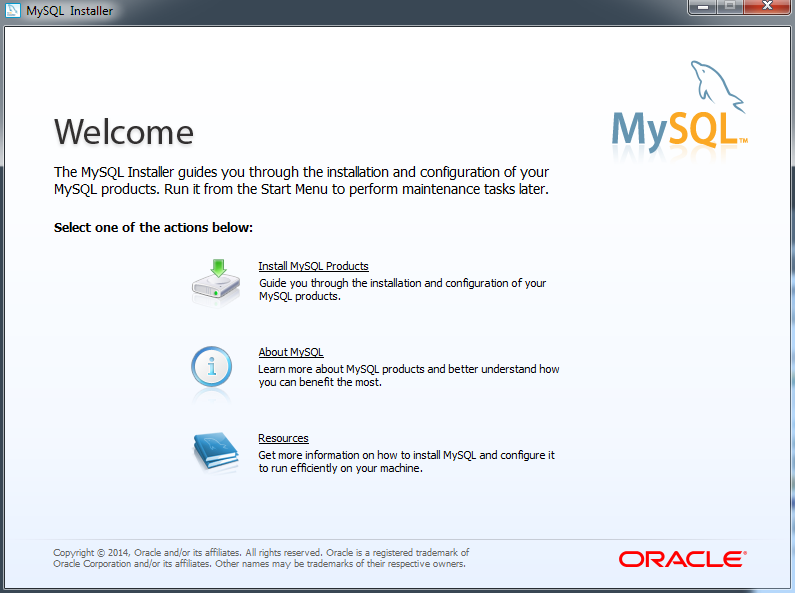
\includegraphics{img/mysql_1.png}
\item
  此时安装程序会尝试联网获取更新,如无 Internet 连接,可以勾选「Skip the
  check for updates」后继续。 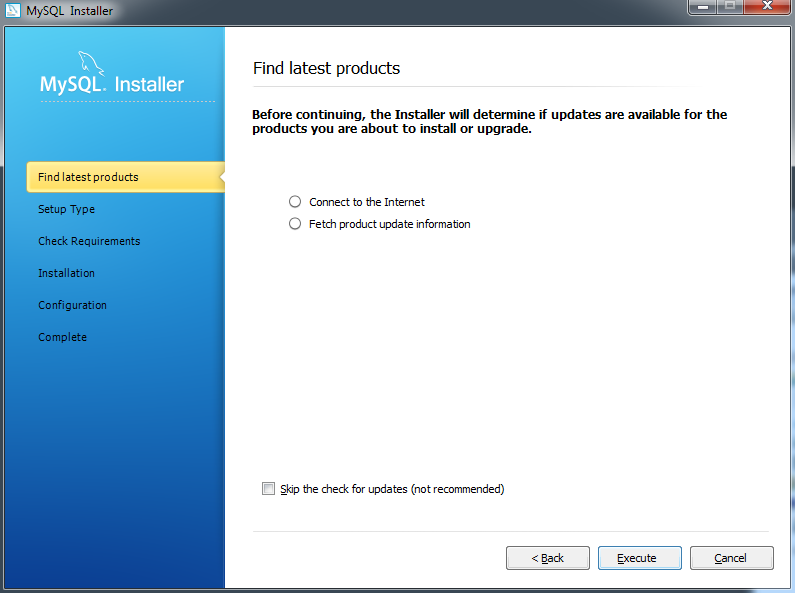
\includegraphics{img/mysql_2.png}
\item
  选择安装类型为「Server only」,并指定数据存放路径。此处我们以
  \texttt{C:\textbackslash{}MySQL\_Data}
  为例,您可以根据具体情况修改该路径。 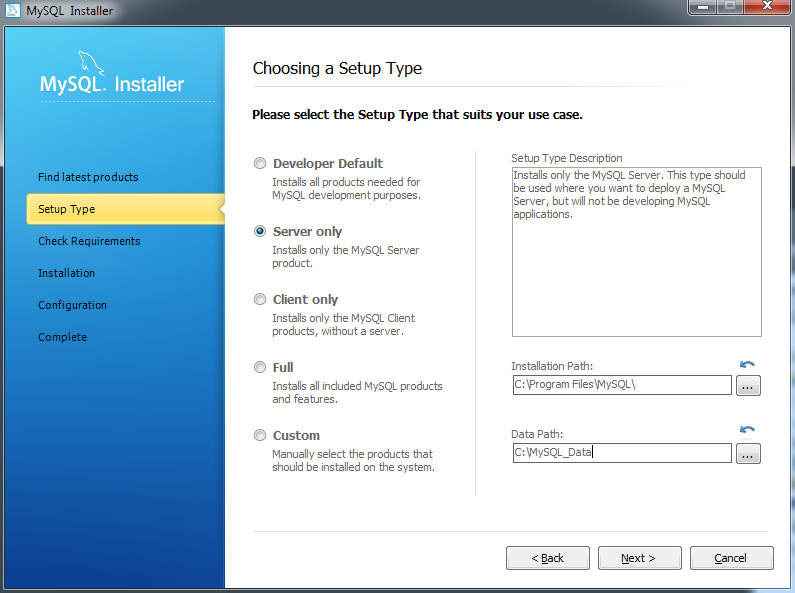
\includegraphics{img/mysql_3.png}
\item
  根据选择的安装项,安装程序检查是否有其他额外的依赖项目需要预先安装。如有,安装程序会下载安装;如无,则可以直接继续。
  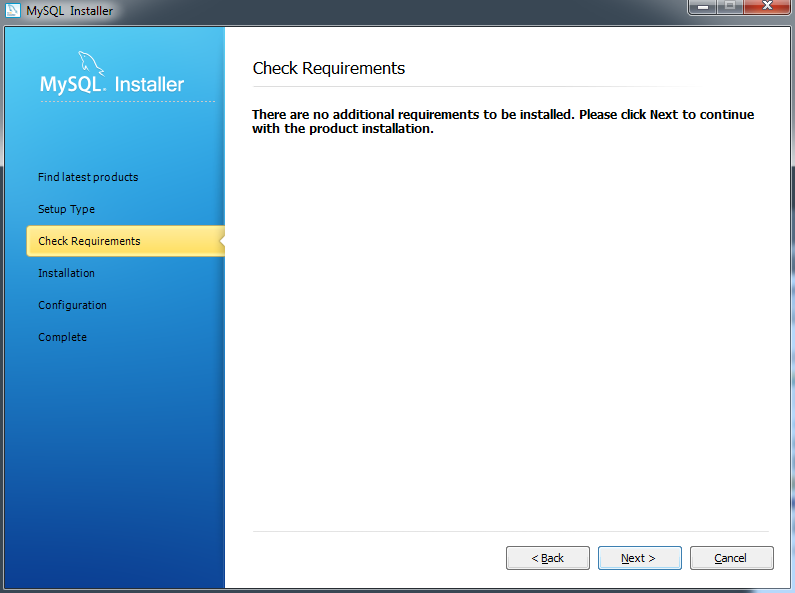
\includegraphics{img/mysql_4.png}
\item
  下面可以安装 MySQL Server 了。点击「Execute」开始安装。
  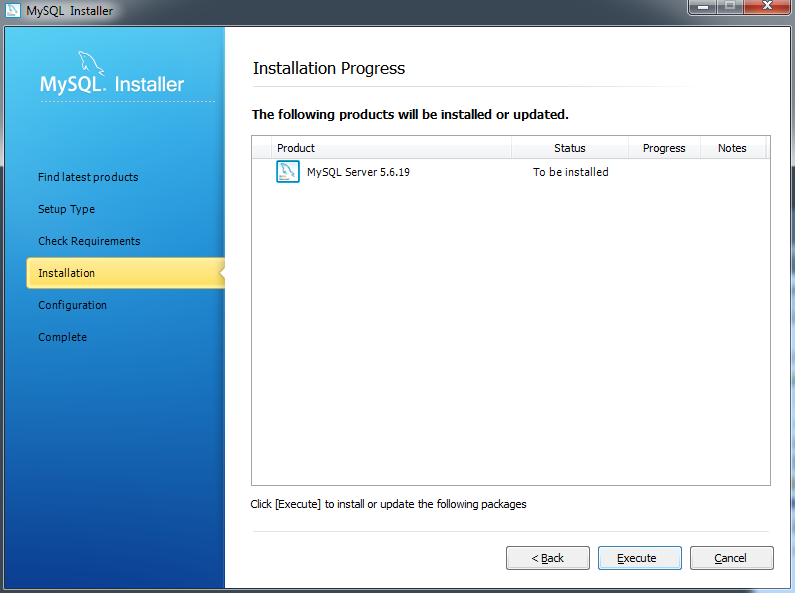
\includegraphics{img/mysql_5.png}
\item
  安装完成后可以进行初始配置,点击「Next」继续。
  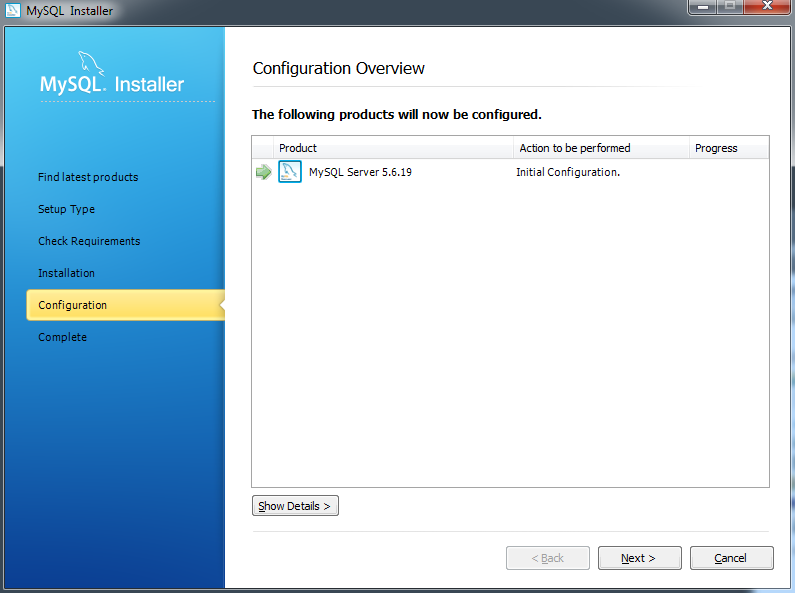
\includegraphics{img/mysql_6.png}
\item
  服务器配置类型选择「Server Machine」并继续。
  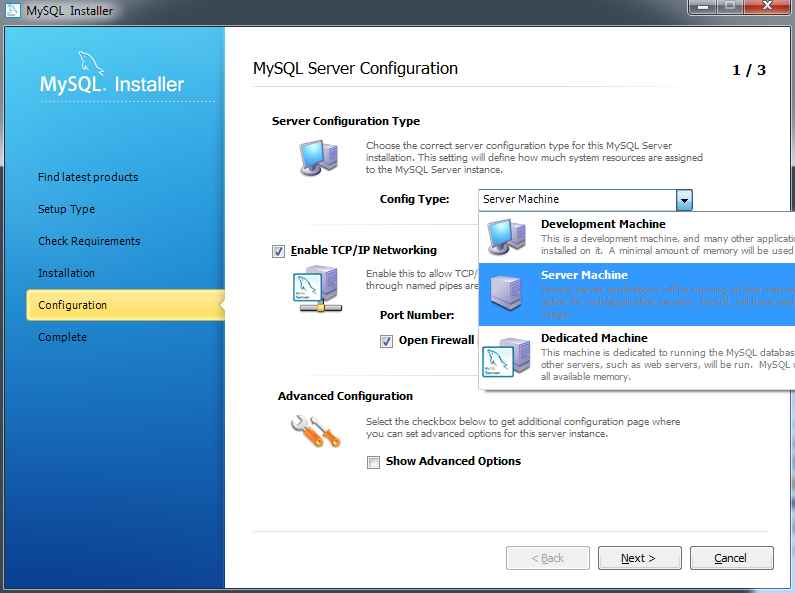
\includegraphics{img/mysql_7.png}
\item
  此处进行用户设置。设置 \texttt{root}
  用户的密码,建议设置复杂密码,并\textbf{请记住此处设置的密码}。单击「Add
  User」新建一个用户作为 StarRiver 的用户。用户名为
  \texttt{sansi},默认密码为
  \texttt{starriver}。\textbf{如您需要修改默认密码,请记住您设置的新密码,后续的配置需要用到这个密码。}
  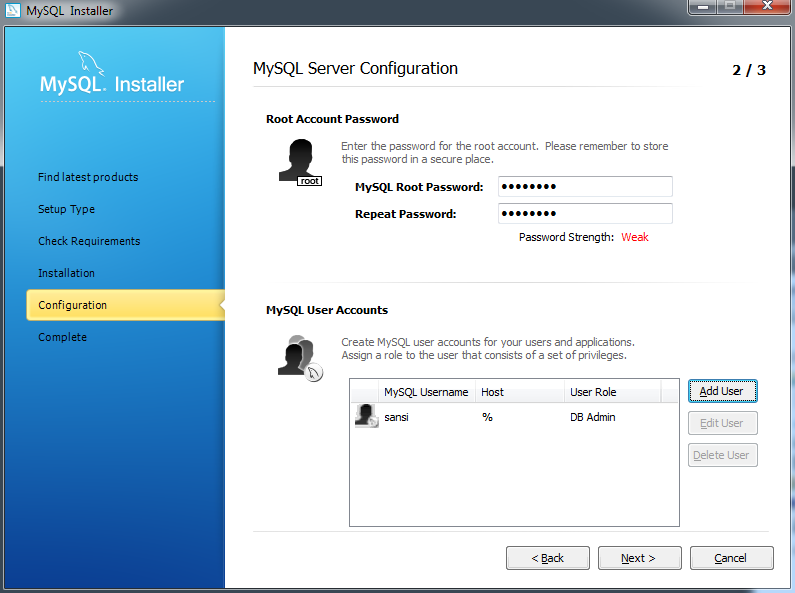
\includegraphics{img/mysql_8.png}
\item
  MySQL Server 将作为 Windows 服务启动,这里我们接受默认设置即可。
  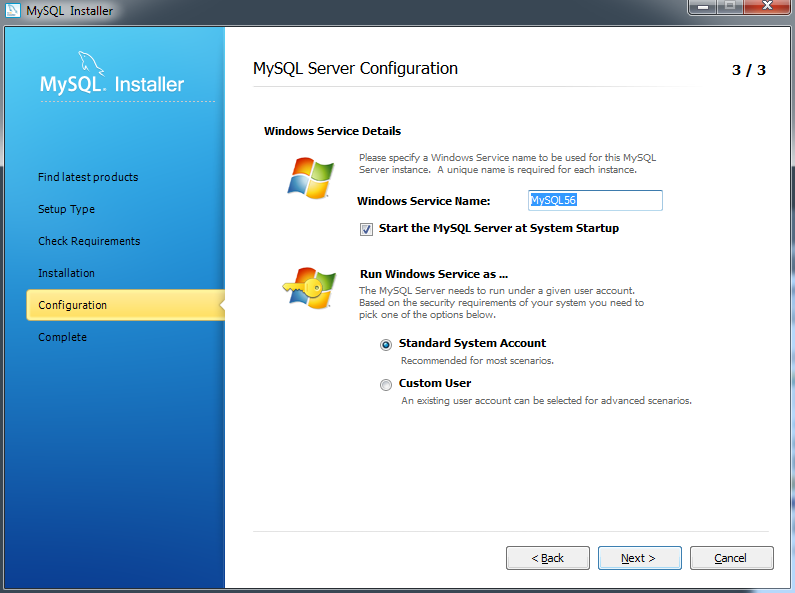
\includegraphics{img/mysql_9.png}
\item
  安装程序配置完成之后,点击「Next」继续。
  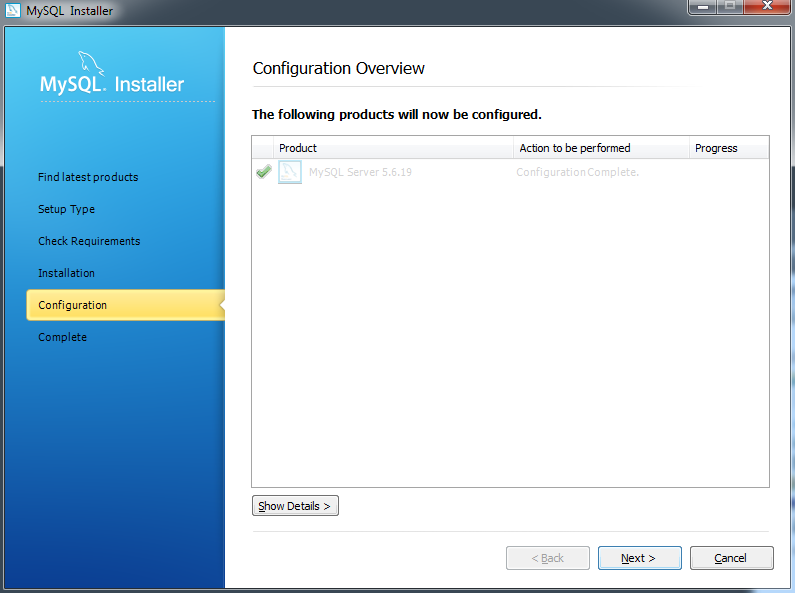
\includegraphics{img/mysql_10.png}
\item
  安装完成。 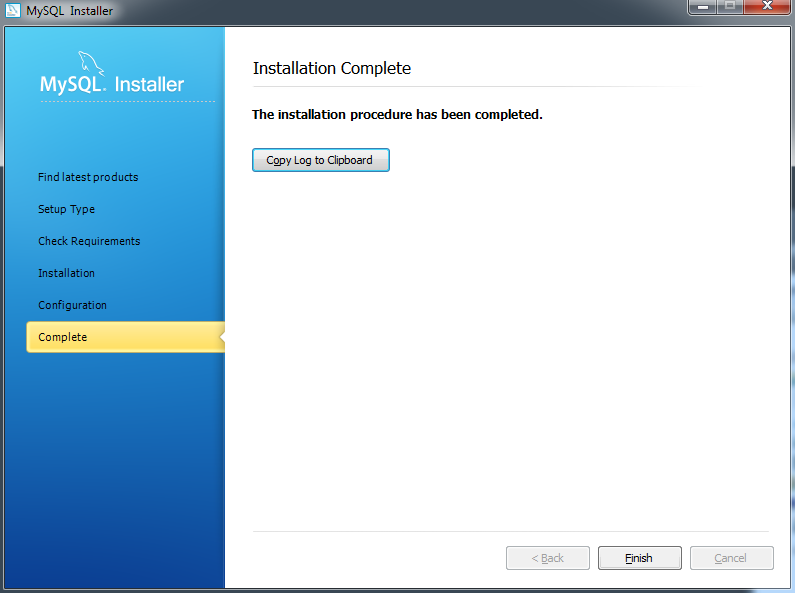
\includegraphics{img/mysql_11.png}
\end{enumerate}

接下来下载安装 \href{http://dev.mysql.com/downloads/workbench/}{MySQL
Workbench},方便我们管理数据库。此处我们采用 MySQL Workbench 6.1.7
版本。安装时全部接受默认选项即可。

最后在 MySQL Workbench 中,建立 StarRiver 需要的数据库表结构。

\begin{enumerate}
\def\labelenumi{\arabic{enumi}.}
\itemsep1pt\parskip0pt\parsep0pt
\item
  打开 MySQL Workbench,单击「MySQL
  Connections」右侧的「+」,新建一个服务器连接。
  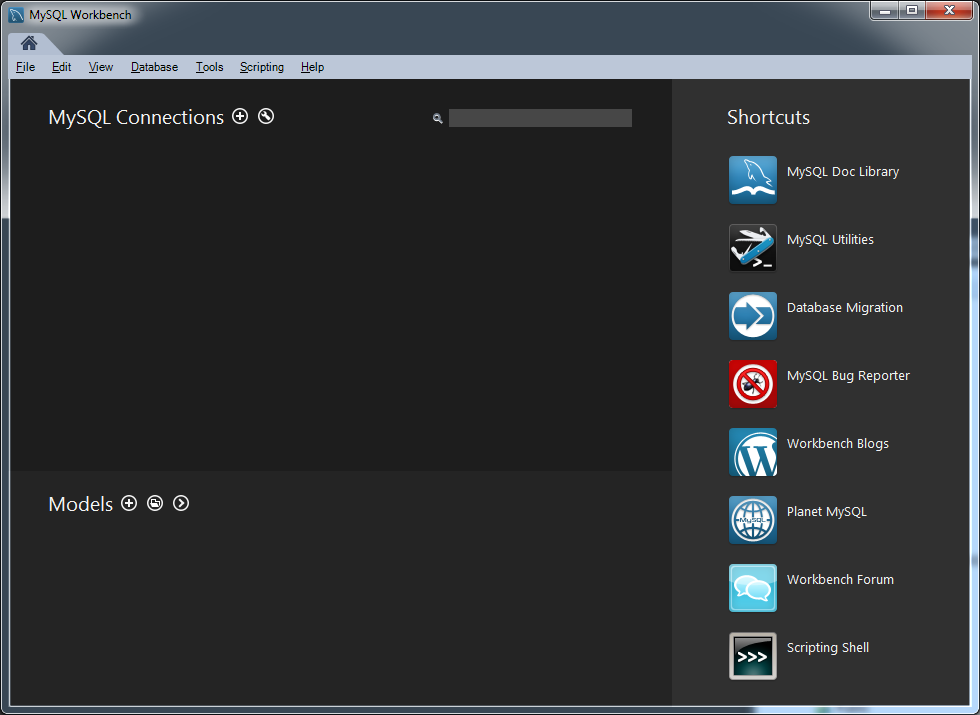
\includegraphics{img/db_init_1.png}
\item
  连接名为「StarRiver」,用户名为 \texttt{sansi},密码单击「Store in
  Vault \ldots{}」并输入 \texttt{starriver}。
  (如您在配置服务器建立用户时未使用默认密码,请输入您自定义的密码。)
  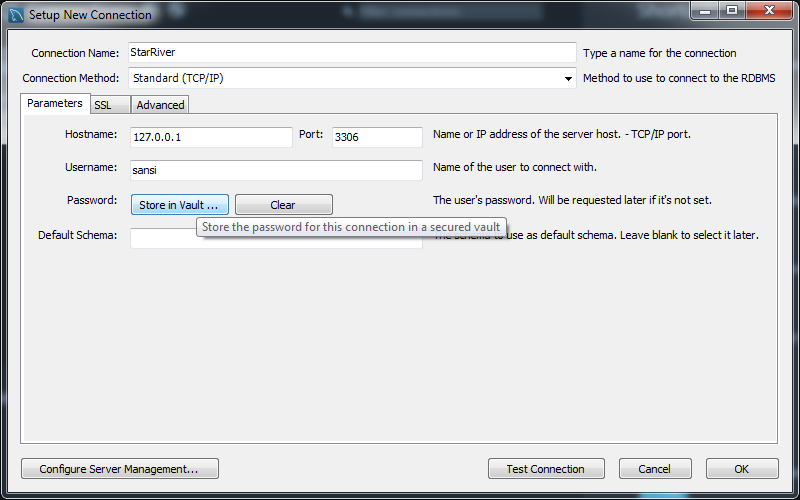
\includegraphics{img/db_init_2.png}
  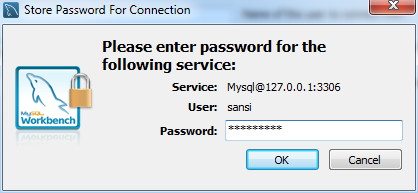
\includegraphics{img/db_init_3.png} 单击「Test
  Connection」,提示连接成功即可。如果报错则说明此前输入有误,请检查输入的用户名、密码等。
  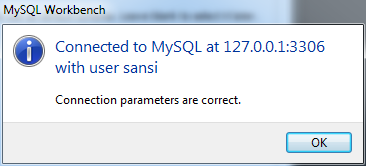
\includegraphics{img/db_init_4.png}
\item
  刚才新建的连接出现在界面上,单击它发起连接。
  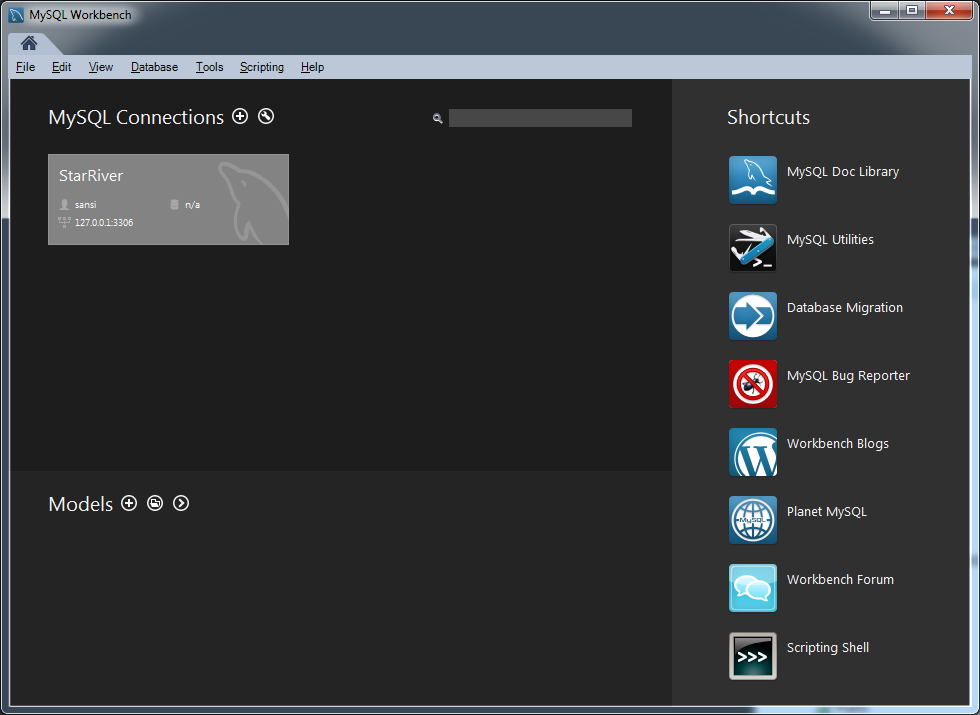
\includegraphics{img/db_init_5.png}
\item
  选择「File-\textgreater{}Open SQL Script」。
  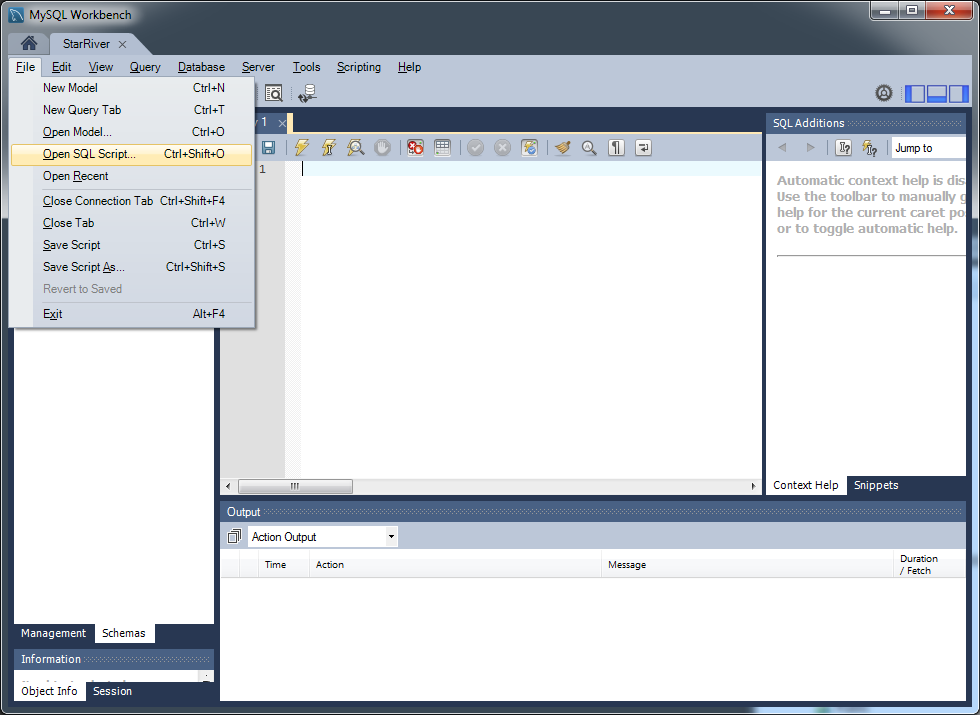
\includegraphics{img/db_init_6.png}
\item
  打开 \texttt{init\_db.sql},单击图中框出的按钮执行脚本。
  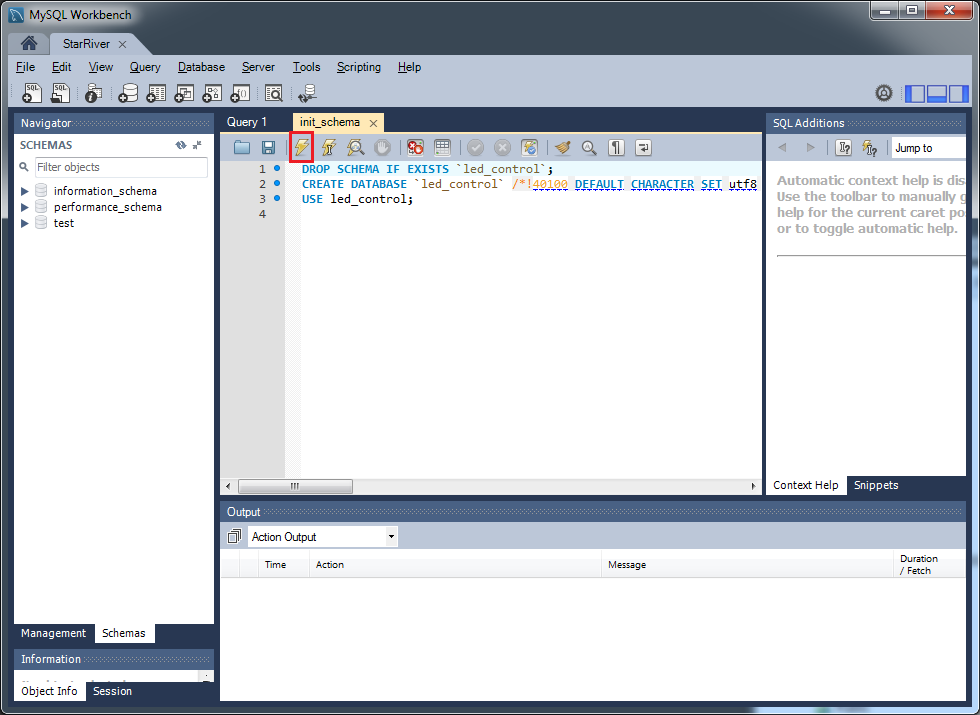
\includegraphics{img/db_init_7.png}
\item
  执行完毕,没有出错。 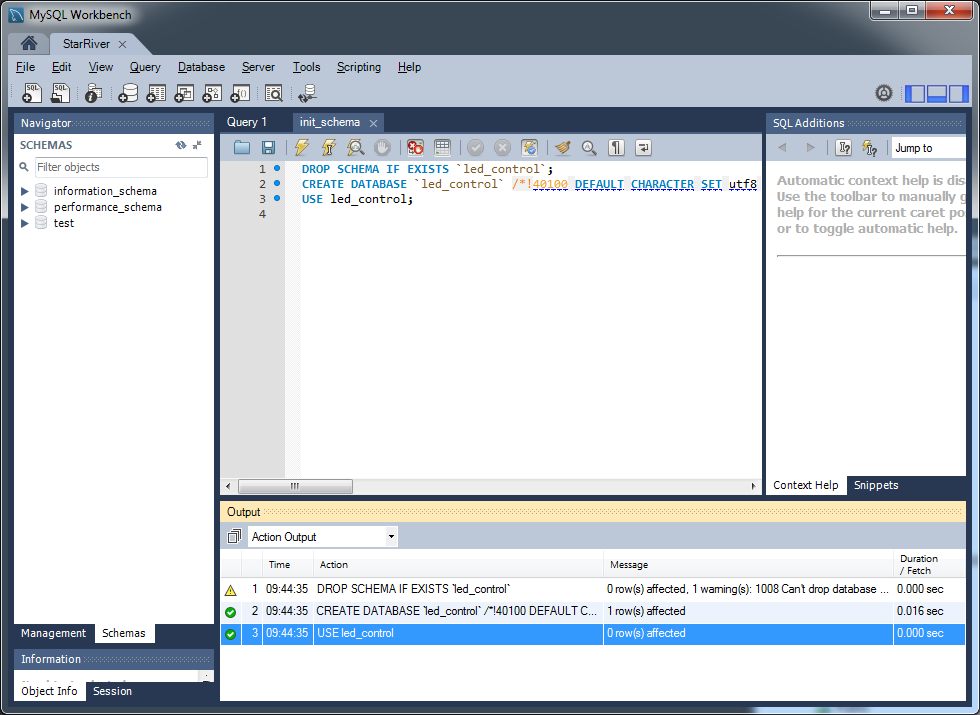
\includegraphics{img/db_init_8.png}
\item
  同样方式打开 \texttt{events.sql},并执行。
  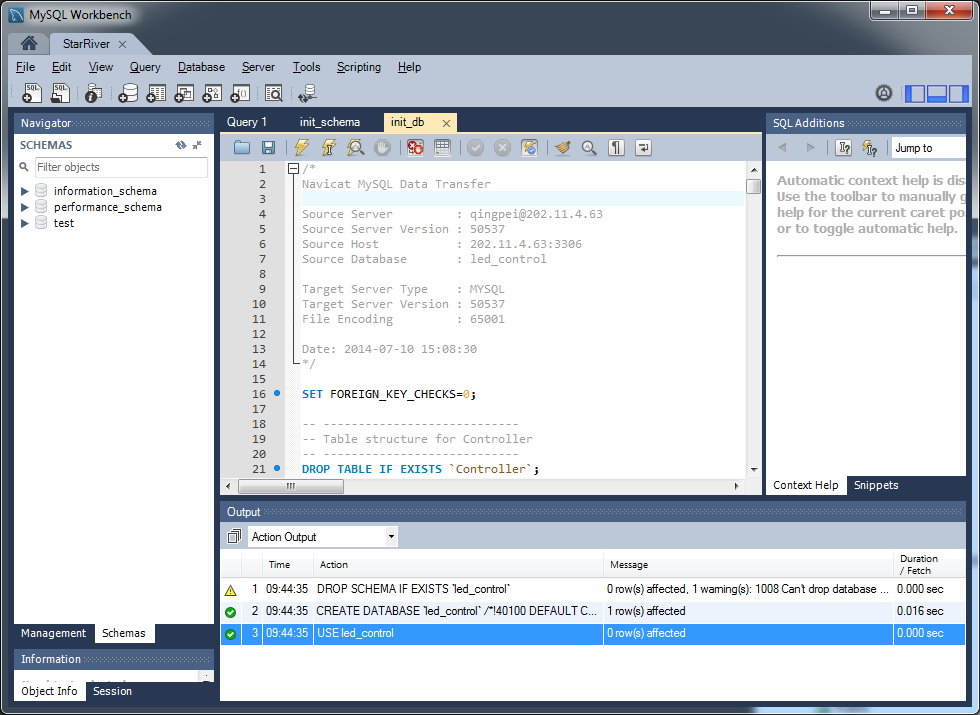
\includegraphics{img/db_init_9.png}
\item
  检查「Output」,没有出错。 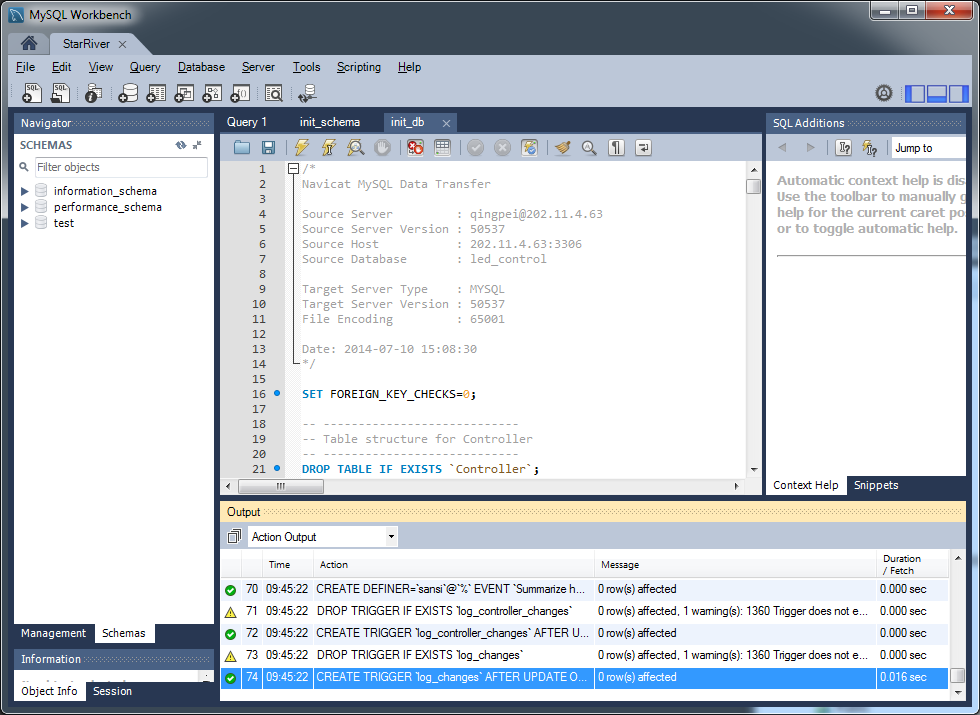
\includegraphics{img/db_init_10.png}
\item
  在左侧「Schemas」窗口内单击刷新按钮,看到名为 \texttt{led\_control}
  的数据库已经被成功建立。 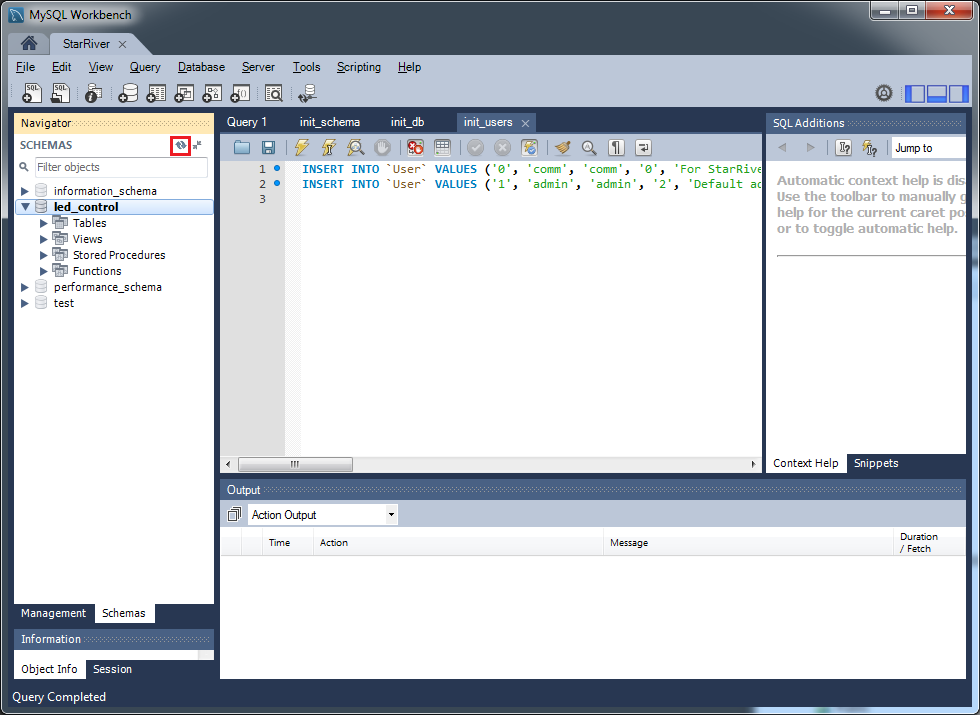
\includegraphics{img/db_init_12.png}
\end{enumerate}

对数据库服务器,还需进行一些配置,方法是修改 MySQL 数据存放路径(前文用
\texttt{C:\textbackslash{}MySQL\_Data} 为例)中的 \texttt{my.ini}。

\begin{figure}[htbp]
\centering
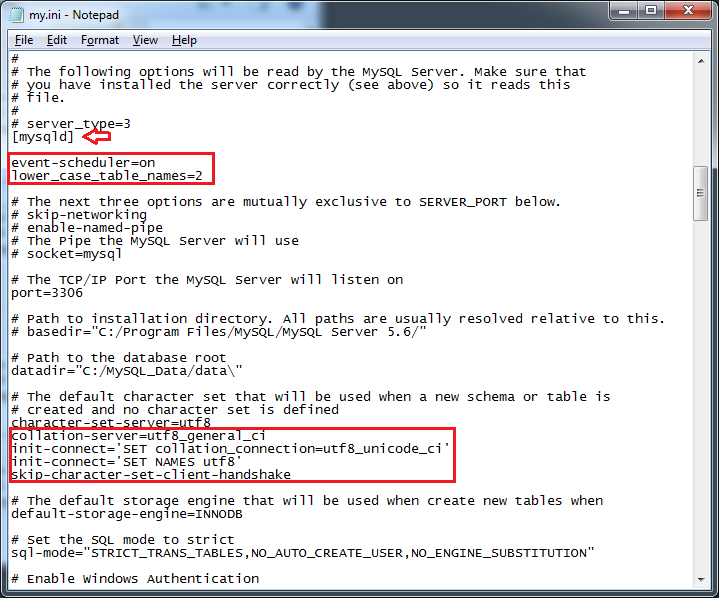
\includegraphics{img/my_ini.png}
\caption{}
\end{figure}

在 \texttt{{[}mysqld{]}} (图中箭头所示)下增加如下内容:

\begin{verbatim}
event-scheduler=on
lower_case_table_names=2

collation-server=utf8_general_ci
init-connect='SET collation_connection=utf8_unicode_ci'
init-connect='SET NAMES utf8'
skip-character-set-client-handshake
\end{verbatim}

\textbf{注意全部是英文单引号\texttt{\textquotesingle{}}}。

重启系统后(或重启 MySQL 服务后),新设置生效。

\subsection{安装 StarRiver
服务}\label{ux5b89ux88c5-starriver-ux670dux52a1}

运行 \texttt{setup.exe}
即可,如需自定义安装路径,请在「目的地文件夹」步骤更改。

\begin{figure}[htbp]
\centering
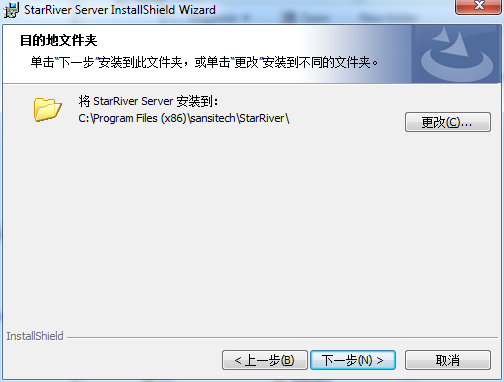
\includegraphics{img/setup.png}
\caption{}
\end{figure}

如您在数据库配置时,未使用本文档提供的默认密码,您还需更改配置文件,让
StarRiver 服务器能够顺利连接数据库。配置文件为安装路径下的
\texttt{config.ini}。

\begin{figure}[htbp]
\centering
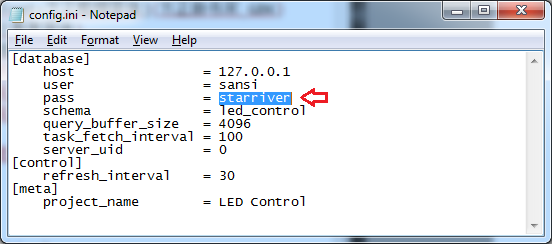
\includegraphics{img/config.png}
\caption{}
\end{figure}

您只需将默认密码(图中箭头所示)改为您此前设置的密码即可。
